%versi 2 (8-10-2016)
 \chapter{Landasan Teori}
\label{chap:teori}

\section{Trajektori}
\label{sec:trajektori}
Trajektori adalah lintasan yang dibuat oleh sebuah objek yang sedang bergerak pada sebuah bidang selama periode waktu tertentu. Istilah trajektori juga digunakan untuk menjelaskan data pergerakan sebuah objek yang sedang bergerak. Trajektori dapat dimodelkan dengan model data atau model abstrak.
 
\par Pada model abstrak, trajektori adalah representasi dari sebuah objek yang sedang bergerak. Objek tersebut diasumsikan sebagai sebuah titik yang bergerak tanpa terputus. Dengan model ini, posisi spasial objek tersebut bisa ditemukan kapan saja. Trajektori dapat dinyatakan sebagai sebuah fungsi yang memetakan interval waktu ke ruang tempat objek bergerak. Pada model tersebut, lintasan dari sebuah trajektori adalah gambaran dari fungsi yang memiliki bentuk dan arah namun tidak memiliki komponen waktu. Data pergerakan umumnya dikumpulkan oleh alat pelacak yang memberikan informasi spasial pada waktu tertentu ketika sampel lokasi objek diambil. Karena keterbatasan teknologi, alat pelacak biasanya melaporkan lokasi pada saat-saat tertentu yang dipisahkan oleh interval waktu yang bersifat regular atau nonregular meskipun pergerakan objek seringkali bersifat kontinu. Karenanya, pada model data, trajektori didefinisikan sebagai rangkaian lokasi, yang terurut berdasarkan waktu, tempat posisi objek bergerak dicatat. Pada model ini ketepatan geometrik dan \textit{sampling rate} mempengaruhi kualitas data trajektori yang dihasilkan. Perbedaan antara model data dengan model abstrak ditunjukkan oleh gambar \ref{fig:model} \cite{wiratma:19:computations}.

\begin{figure}[H]
	\centering  
	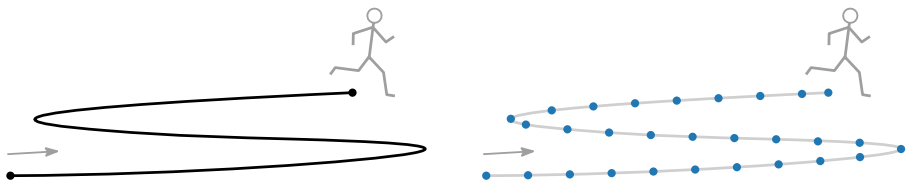
\includegraphics[scale=0.5]{trajektori}  
	\caption{Ilustrasi model abstrak (kiri) dan model data (kanan) pada trajektori} 
	\label{fig:model} 
\end{figure}

\subsection{Ruang Gerak}
Terdapat beberapa jenis ruang gerak tempat sebuah objek bergerak. Jenis ruang gerak ditentukan oleh jenis objek yang diamati dan jenis aplikasi atau program yang menggunakan data pergerakan. Jika tinggi atau kedalaman sebuah posisi dianggap tidak penting, maka ruang gerak yang digunakan adalah bidang euclidean $\mathbb{R}^{2}$. Jika sebaliknya, maka ruang gerak yang digunakan adalah bidang euclidean $\mathbb{R}^{3}$ \cite{wiratma:19:computations}.

\subsection{Persepektif Lagrangian atau Eulerian}
Terdapat dua pendekatan untuk mengekstrak data trajektori untuk model dat. Menurut persepektif langrangian, data trajektori diperoleh dengan melacak posisi objek saat objek tersebut bergerak selama durasi tertentu. Metode ini berguna untuk mendapatkan detail gerakan objek. Persepektif lagrangian disebut juga persepektif berbasis objek. Berbeda dengan persepektif lagrangian, persepektif elulerian bersifat berbasis lokasi. Persepektif ini berfokus kepada proses observasi gerakan objek dari lokasi tertentu dengan memanfaatkan teknologi seperti \textit{tag} RFID, jaringan WiFi, atau jaringan GSM. Perbedaan persepektif lagrangian dan eulerian ditunjukkan oleh gambar \ref{fig:eula} \cite{wiratma:19:computations}.
\begin{figure}[H]
	\centering  
	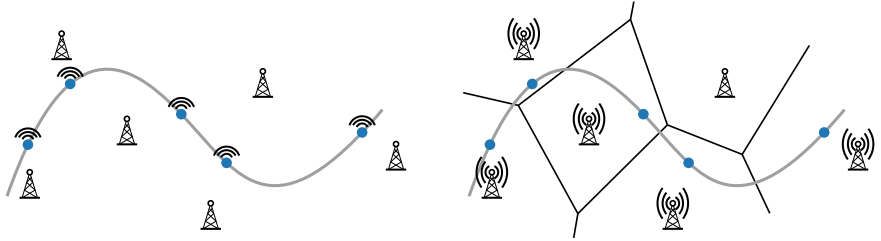
\includegraphics[scale=0.5]{eula}  
	\caption{Ilustrasi persepektif lagrangian (kiri) dan persepektif eulerian (kanan) pada pergerakan sebuah benda. Pada persepektif lagrangian, data pergerakan benda dikumpulkan selama benda berwarna biru bergerak menyusuri lintasan abu-abu. Informasi berupa rekaman lokasi-lokasi diperoleh dari alat pelacak yang terpasang pada benda. Pada persepektif eulerian, pergerakan benda dilacak dari lokasi tertentu.} 
	\label{fig:eula} 
\end{figure}

\subsection{Interpolasi Trajektori}
Meskipun mengumpulkan data trajektori dengan menggunakan metode lagrangian memungkinkan pengambilan sampel trajektori dengan resolusi spasial yang bagus, manfaat utama data trajektori bergantung kepada skala yang digunakan pada proses analisis atau aplikasi yang memanfaatkan data tersebut. Jika menggunakan skala yang lebih besar, maka mungkin saja posisi objek pada selang waktu yang terletak di antara dua sampel tidak diketahui. Namun, karena pergerakan benda bersifat kontinu, data trajektori yang bersifat diskrit harus dianalisa dan diproses dalam bentuk kontinu. Terdapar beberapa metode untuk menyelesaikan masalah ini.
\par Metode pertama adalah mengacuhkan masalah ini dan hanya menganalisa trajektori pada waktu saat lokasi diketahui. Keunggulan metode ini adalah dapat memproses data trajektori secara ringkas dan cepat. Namun, jika data trajektori tidak di-\textit{sampling} dengan jumlah sampel yang mencukupi, maka lokasi dan waktu yang terletak di antara dua rekaman lokasi dapat diperoleh melalui proses interpolasi. Asumsi paling sederhana untuk lokasi dari sebuah objek yang bergerak pada waktu yang terletak di antara dua titik sampel yang terletak berurutan adalah dengan melakukan interpolasi linear pada dua lokasi tersebut. 
\par Pada interpolasi tersebut, benda yang dapat bergerak diasumsikan bergerak dengan kecepatan konstan pada garis lurus yang menghubungkan kedua lokasi. Jika data trajektori disampel dengan jumlah yang mencukupi, interpolasi ini bisa dianggap tidak memiliki \textit{error} yang signifikan. Metode ini sangat umum digunakan pada bidang GIS(\textit{Geographic Information System}), \textit{computational geometry}, dan domain lainnya. Kadangkala, interpolasi linear tidak bersifat realistis pada sejumlah permasalahan. Sehingga dibutuhkan metode interpolasi yang lebih kompleks \cite{wiratma:19:computations}.
\begin{figure}[H]
	\centering  
	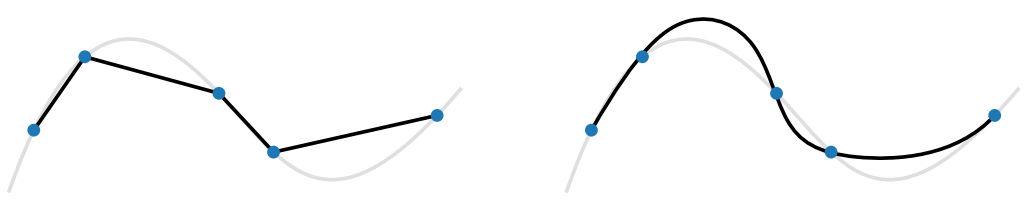
\includegraphics[scale=0.5]{intp}  
	\caption{Trajektori sungguhan sebuah objek (garis abu-abu) dan perbedaan hasil interpolasi pada data berupa urutan lokasi objek (lingkaran-lingkaran berwarna biru). Setiap lokasi memiliki atribut waktu. Pada interpolasi linear (kiri), objek tersebut diasumsikan bergerak pada lintasan lurus yang terletak di antara dua lingkaran dengan kecepatan tetap. Pada interpolasi nonlinear (kanan), lintasan yang dilalui tidak berbentuk garis lurus} 
	\label{fig:interp} 
\end{figure}

\subsection{Notasi}
Misalkan $T$ adalah trajektori sebuah entitas. Pada model abstrak, trajektori adalah sebuah fungsi yang memetakan sebuah interval waktu $I=[t_{\alpha},t_{\beta}]$ ke ruang. Lokasi pada waktu mulai $t_{\alpha}(t_{start})$ adalah pangkal trajektori $T$ dan lokasi pada waktu akhir $t_{\beta}(t_{end})$ adalah tujuan trajektori $T$. 
\par Pada model abstrak, trajektori terdiri dari urutan lokasi yang masing-masing memiliki atribut waktu (\textit{timestamp}) $(p_{1},t_{1}),(p_{2},t_{2}),\cdots,(p_{r},t_{r})$ dengan $p_{i}=(x_{i},y_{i})$ menyatakan posisi objek pada waktu  $t_{i}$ dan $r$ menyatakan banyaknya data yang dicatat \cite{wiratma:19:computations}.

\subsection{Data Trajektori}
Data trajektori berasal dari berbagai benda bergerak, contohnya kendaraan, binatang, dan pejalan kaki. Terdapat beragam metode untuk mendapatkan data trajektori benda-benda tersebut. Kualitas data yang diperoleh dipengaruhi oleh beberapa faktor seperti jenis benda, lingkungan tempat observasi dilakukan, teknologi yang digunakan, dan lainnya.

\par Data trajektori dapat diperoleh secara manual atau dengan memanfaatkan teknologi tertentu. Keunggulan metode manual adalah tidak membutuhkan sumber tenaga eksternal. Namun, metode ini memiliki beberapa kelemahan yaitu rendahnya kepresisian dari lokasi-lokasi yang diperoleh dan banyaknya data trajektori yang dapat diperoleh terbatas. Metode berbasis teknologi digunakan untuk memperoleh data trajektori dengan presisi yang tinggi dalam skala besar untuk durasi waktu lebih lama. Contohnya adalah teknologi \textit{VHF Radio Telemetry, argos-doppler system}, dan GPS. Secara umum terdapat dua jenis alat yang digunakan yaitu alat pemancar(\textit{transmitter}) atau alat penerima (\textit{receiver}). Alat tersebut dipasang pada objek yang diobservasi trajektorinya. Pada lingkungan dengan ukuran terbatas (misalnya, didalam bangunan), alat yang digunakan adalah alat yang dikhususkan untuk lingkungan tersebut seperti sensor, bluetooth, sensor jangkauan 3D statis, dan lainnya.

\par Kualitas data trajektori yang bisa diperoleh dengan menggunakan alat-alat tersebut bergantung pada beberapa faktor seperti cuaca, kekuatan baterai, dan kekuatan sinyal. Sehingga data trajektori yang diperoleh, contohnya pada dua lokasi yang berurutan, mungkin saja tidak memiliki interval waktu yang seragam. Masalah yang hampir serupa juga muncul pada trajektori yang diperoleh dari kumpulan benda bergerak; interval waktu yang tercatat mungkin berbeda-beda.

\par Kadangkala alat pelacak sangat sulit untuk digunakan di beberapa lingkungan. Untuk mengatasi masalah ini, pergerakan objek bisa direkam menggunakan kamera video. Lalu data trajektori diekstrak dari rekaman video menggunakan algoritma tertentu. Contoh implementasi metode ini adalah trajektori ikan di lautan atau trajektori pejalan kaki di dalam maupun di luar ruangan.

\par Jika data trajektori sulit diperoleh dengan menggunakan salah satu dari metode-metode sebelumnya, maka pergerakan dari objek bergerak dapat dimodelkan  menggunakan metode tertentu. Trajektori diperoleh dari hasil simulasi program komputer yang mengimplementasikan model yang dibuat sebelumnya. Data yang dihasilkan disebut data trajektori artifisial. Meskipun proses memodelkan gerakan benda-benda cukup rumit, Metode ini memiliki keunggulan dibandingkan dengan metode sebelumnya yaitu parameter-parameter penting simulasi dapat diatur contohnya: durasi simulasi, ukuran dan jenis lingkungan, jumlah benda pada lingkungan, dan atribut-atribut benda bergerak (kecepatan,perilaku) \cite{wiratma:19:computations}.

\section{Analisis Trajektori}
Terdapat sejumlah metode yang baru-baru ini dikembangkan untuk menganalisis data trajektori. Metode-metode tersebut adalah segmentasi, \textit{similarity determination}, \textit{clustering}, representasi, dan berbagai jenis \textit{pattern} yang mungkin muncul dari gerakan benda-benda.

\subsection{Similaritas}
Analisa similaritas bertujuan untuk menentukan apakah dua trajektori terlihat serupa atau tidak. Kemiripan dua trajektori ditentukan oleh berbagai jenis definisi seperti mengunjungi lokasi yang sama, atau memiliki perubahan kecepatan yang sama (misalnya pelan diawal, cepat diakhir). Analisa similaritas juga  digunakan untuk \textit{preprocessing} atau sebagai \textit{subroutine} untuk metode analisa lain.

\par Similaritas pada dua buah trajektori kadang ditentukan oleh jarak diantara dua trajektori tersebut. Terdapat beberapa metode pengukuran jarak untuk menentukan similaritas trajektori. Jika hanya lintasan trajektori yang dianggap penting, maka metode yang digunakan adalah \textit{euclidean distance, hausdorff distance}, atau \textit{frechet distance}. Metode pengukuran lain mengolah aspek temporal trajektori. Contohnya adalah \textit{Dynamic Time Warping, time-focused distance, edit distance}, dan \textit{longest common subsequence}. Atribut tambahan pada gerakan seperti kecepatan, percepatan, dan arah gerakan bisa digunakan untuk menentukan similaritas.

\subsection{Clustering}
\textit{Clustering} adalah proses mempartisi sebuah objek menjadi beberapa \textit{cluster}. Objek-objek yang berada pada \textit{cluster} yang sama memiliki sifat yang mirip tetapi berbeda dengan objek anggota \textit{cluster} lain. \textit{Clustering} dapat diterapkan pada trajektori yang berasal dari beberapa objek. Trajektori dapat dibagi ke dalam beberapa \textit{cluster} berdasarkan similaritas antar trajektori atau subtrajektori. \textit{Clustering} pada trajektori dapat digunakan untuk mendeteksi \textit{movement pattern} tertentu.

\subsection{Representasi}
Sebuah \textit{cluster} yang berisi trajektori dapat direpresentasikan oleh sebuah trajektori yang dipilih menggunakan metode tertentu. Trajektori tersebut dapat merepresentasikan beberapa hal seperti rute yang ditempuh oleh sebuah benda, atau pergerakan benda tertentu. Gambar \ref{fig:repr} mengilustrasikan  beberapa contoh trajektori representatif yang mungkin dari sebuah \textit{cluster}.
\begin{figure}[h]
	\centering  
	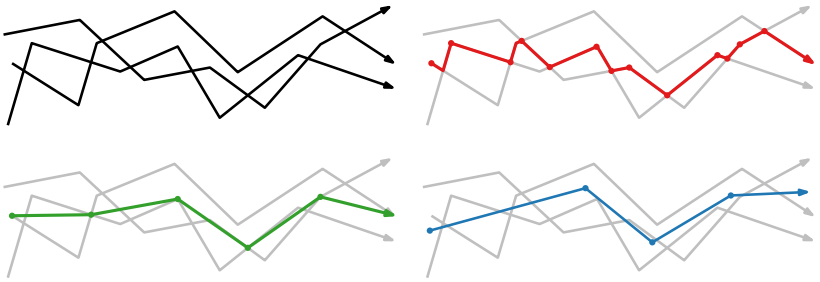
\includegraphics[scale=0.5]{repr}  
	\caption{Contoh trajektori yang merepresentasikan sebuah kumpulan trajektori yang berwarna hitam (kiri atas). Terdapat tiga trajektori representatif yaitu trajektori berwarna merah yang menggunakan bagian dari kumpulan trajektori (kanan atas), trajektori berwarna hijau yang menggunakan verteks pada himpunan trajektori(kiri bawah), dan membentuk sebuah trajektori baru (trajektori warna biru, kanan bawah)} 
	\label{fig:repr} 
\end{figure}

\par Trajektori representatif memiliki beberapa manfaat. Pertama, mengurangi jumlah data trajektori yang perlu dianalisis karena trajektori tersebut sudah merpresentasikan trajektori lain yang serupa. Kedua, trajektori representatif memiliki visualisasi yang lebih baik karena lebih berfokus ke satu atau sedikit trajektori. Ketiga, untuk menemukan \textit{outlier} dengan cara menganalisis similaritas atau \textit{closeness} antara trajektori representatif dengan trajektori lainnya.

\subsection{Movement Patterns}
\textit{Movement pattern} sebuah objek adalah atribut-atribut yang diperoleh dari trajektori objek tersebut. Pada kumpulan objek yang bergerak, \textit{movement pattern} mengacu pada interaksi atau relasi antar objek. Karena setiap jenis benda bergerak memiliki tipe relasi dan atribut yang berbeda-beda, \textit{pattern-pattern} yang nampak pada benda-benda tersebut juga berbeda-beda. Contohnya, pola gerakan pengunjung di taman bisa saja mengandung informasi tempat-tempat menarik yang sering dikunjungi.

\par Pada trajektori tunggal, pola gerakan yang umum ditemui adalah \textit{periodic pattern, commmuting}, dan \textit{concentration pattern}. Sedangkan pada sepasang trajektori, pola gerakan yang kerap kali ditemui adalah \textit{chasing behavior} dan \textit{avoidance movement}. Pada kumpulan trajektori, pola gerakannya adalah \textit{leadership pattern, meeting pattern, convergence pattern}, dan lainnya. Contoh pattern tersebut ditunjukkan oleh gambar  \ref{fig:poger}.
\begin{figure}[h]
	\centering  
	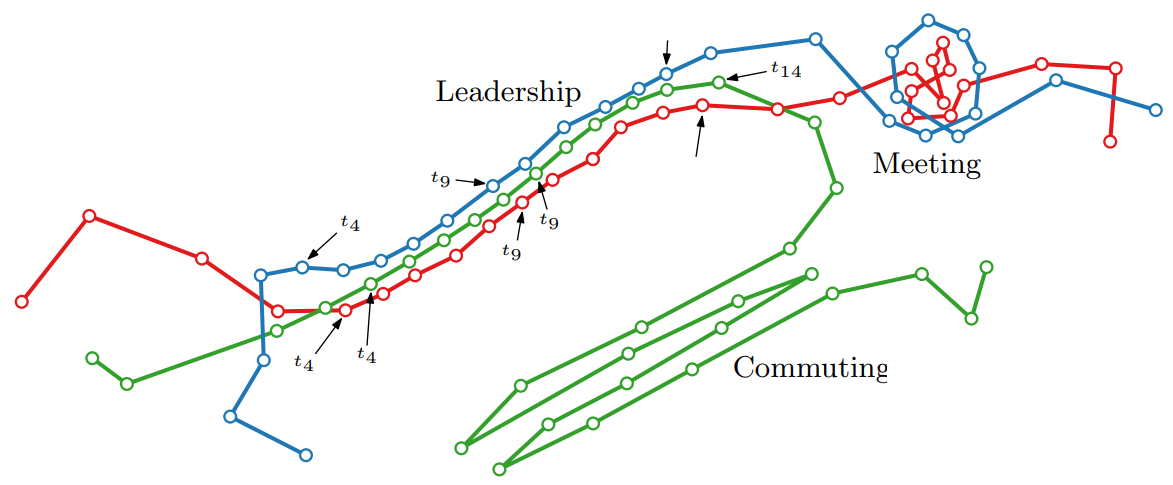
\includegraphics[scale=0.5]{poger}  
	\caption{Tiga trajektori dengan tiga jenis \textit{pattern} yang ditunjukkan pada gambar. Pada selang waktu antara $t_{4}$ hingga $t_{14}$, benda berwarna hijau menjadi pemimpin (\textit{leader}) dan diikuti oleh dua benda lainnya, yaitu biru dan merah.} 
	\label{fig:poger} 
\end{figure}

\section{Collective Motion}
\label{sec:collmotion} 
 
\par \textit{Collective motion} adalah kemunculan gerakan teratur yang terjadi secara spontan pada sistem yang terdiri dari beberapa \textit{self-proplelled-agent} \cite{palacci:13:living}. Fenomena tersebut dapat ditemukan pada perilaku makhluk hidup contohnya pada kawanan ikan, burung, atau kerumunan orang yang merupakan hasil interaksi lokal antara individu-individu pada proses swaorganisasi (self-organization). Swaorganisasi adalah proses untuk mencapai tujuan tertentu dengan cara mengatur perilaku antar individu secara mandiri \cite{wilshaw:06}.

\par \textit{Collective motion} adalah salah satu jenis \textit{pattern} yang sudah dipelajari dalam beberapa metode. Istilah \textit{collective movement} kadang disebut \textit{group}. \textit{Collective motion} memiliki hubungan dengan \textit{clustering}. Namun \textit{clustering} berbeda dengan \textit{collective motion}. Pada \textit{clustering}, seluruh trajektori dilibatkan pada proses pembuatan \textit{cluster}. Pada \textit{collective motion}, sebuah benda bisa menjadi anggota \textit{group} yang berbeda pada waktu yang berbeda atau pada waktu yang sama. Terdapat beberapa aspek yang harus diperhatikan pada pemodelan \textit{collective movement}, yaitu:

\begin{enumerate}
\item \textit{Input trajectories}\\
Data gerakan (\textit{movement data}) dikumpulkan dalam bentuk trajektori diskrit (urutan lokasi-lokasi yang memiliki atribut waktu) dan data tersebut dapat diubah ke bentuk kontinu dengan menggunakan interpolasi. Jika model \textit{collective motion} hanya memproses data dalam bentuk diskrit, maka waktu mulai dan waktu akhir sebuah \textit{group} harus sesuai dengan catatan waktu yang direkam pada data trajektori. Jika menggunakan data dalam bentuk kontinu, maka waktu dan posisi benda-benda di antara lokasi-lokasi yang diketahui dapat diestimasi. Karena itu, \textit{group} yang sama mungkin memiliki interval waktu yang lebih panjang karena perbedaan pada waktu awal dan / atau waktu akhir.

\item \textit{Spatial proximity}\\
Umumnya, benda-benda yang bergerak bersama-sama memiliki posisi yang saling berdekatan. Definisi \textit{closeness} yang paling sederhana adalah sebuah variabel $\epsilon > 0$ yang menyatakan jarak maksimum di antara dua benda. Definisi tersebut lalu dikembangkan untuk mengakomodasi \textit{collective movement}. Pada \textit{collective motion}, setiap pasang benda pada \textit{group} harus terletak sedekat mungkin pada setiap waktu. Terdapat juga definisi \textit{closeness} lain. Menurut Gudmundsson dan van Kreveld \cite{flock_pattern_2:06}, sebuah \textit{group} direpresentasikan oleh sebuah lingkaran dengan jari-jari $\epsilon$ dan objek-objek anggota \textit{group} harus terletak di dalam lingkaran tersebut. Pada metode lainnya, terdapat sebuah objek lain yang menjadi perantara, dua objek $i$ dan $j$ disebut saling berdekatan meskipun $d_{ij}(t) > \epsilon$ selama terdapat objek lain yaitu $k$ sehingga $d_{ik}(t)\leq \epsilon$ dan $d_{kj}(t)\leq \epsilon$.
\begin{figure}[h]
	\centering  
	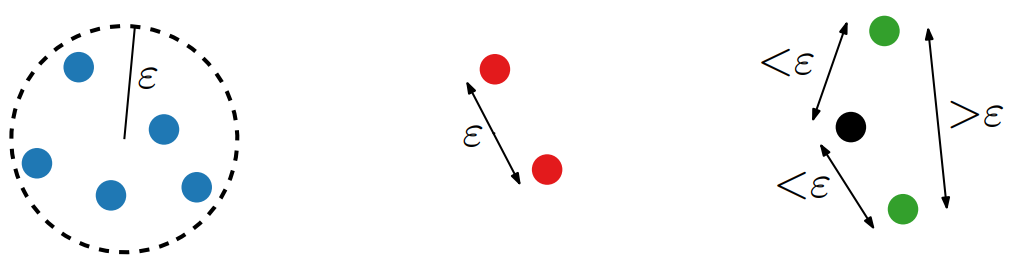
\includegraphics[scale=0.5]{dist}  
	\caption{Jenis-jenis \textit{spatial proximity}. Pada gambar di sebelah kiri, semua objek terletak di dalam sebuah lingkaran dengan jari-jari $\epsilon$. Pada gambar di tengah, jarak dua benda harus tidak lebih dari $\epsilon$. Pada gambar di sebelah kanan, dua objek dianggap berdekatan dengan menggunakan objek berwarna hitam sebagai perantara.} 
	\label{fig:dist} 
\end{figure}

\item \textit{Size}\\
Dua objek yang yang bergerak bersama-sama dapat dianggap sebagai sebuah \textit{group}. Batasan ukuran sebuah \textit{group} dipengaruhi oleh aplikasi yang  digunakan. Selain itu, sebuah objek dapat menjadi anggota satu \textit{group} atau beberapa \textit{group}.

\item \textit{Temporal Component}\\
\textit{Temporal component}  waktu minimal yang dibutuhkan pada kumpulan benda-benda untuk tetap bersama hingga dapat dianggap sebagai \textit{group}. hal paling penting pada durasi sebuah \textit{group} adalah kontinuitas durasi \textit{group} tersebut. 

\end{enumerate}
\par Terdapat bermacam-macam model dari \textit{collective movement} dengan definisi yang sedikit berbeda-beda. Salah satu definisi yang digunakan adalah \textit{flock}. Istilah lain yang berhubungan erat dengan konsep \textit{flock} adalah \textit{micro-cluster, moving cluster, mobile group, herd, convoy, swarm, traveling companion, gathering, platoon}, dan \textit{group}. Seluruh definisi tersebut bergantung pada paling sedikit tiga parameter yaitu: ukuran(\textit{size}), parameter temporal, dan parameter spasial. Mayoritas definisi yang disebutkan menggunakan trajektori yang dimodelkan secara diskrit, namun ada juga yang menggunakan trajektori yang dimodelkan secara kontinu, contohnya \textit{group}.
 
 
\section{\textit{Online Algorithm}}
Pada komputasi online, sebuah algoritma harus menghasilkan keluaran berupa rangkaian keputusan yang memiliki dampak terhadap kualitas akhir dari keseluruhan kinerja algoritma tersebut. Setiap keputusan harus dibuat berdasarkan kejadian-kejadian di masa lalu tanpa informasi yang pasti tentang masa depan. Algoritma yang memiliki ciri-ciri demikian disebut algoritma online (\textit{online algorithms}). Algoritma online adalah topik yang menarik di berbagai bidang ilmu. Banyak masalah komputasi yang bersifat online secara intrinsik sehingga membutuhkan keputusan yang dibuat sesegera mungkin. 
\par Pendekatan tradisional untuk mempelajari algoritma \textit{online} adalah bagian dari \textit{distributional complexity framework}.
 Pada \textit{framework} tersebut, hipotesis tentang distribusi kejadian dibuat dan \textit{total cost} atau \textit{expected cost} setiap kejadian dipelajari. \cite{algo_online_1_8_mar_2021:98}

\par Algoritma \textit{online} adalah jenis algoritma yang menerima rangkaian masukan satu per satu sesuai urutan tibanya dan menghasilkan keluaran untuk setiap masukan sesegera mungkin. Setiap pasangan input dan keluaran yang dihasilkan memiliki \textit{cost} tertentu. Algoritma \textit{online} digunakan pada situasi-situasi yang membutuhkan keputusan instan meskipun data masukan yang dimiliki tidak lengkap.  

\par algoritma \textit{online} memiliki sejumlah perbedaan dengan algoritma \textit{offline}. Pada algoritma \textit{offline}, seluruh masukan yang akan dikerjakan sudah tersedia dari awal. Algoritma \textit{offline} harus melakukan aksi tertentu untuk setiap masukan yang diterima namun, pilihan aksi yang dapat dipilih dapat didasarkan pada seluruh masukan yang ada. Algoritma \textit{offline} dianggap mengetahui masa depan sementara algoritma \textit{online} tidak. Pada banyak keadaan, ketidaktahuan tentang masa depan sangat tidak menguntungkan. Karenanya, algoritma \textit{online} seringkali memiliki kinerja yang lebih buruk dibandingkan dengan algoritma \textit{offline} optimal pada masalah yang sama.

\par Algoritma \textit{offline} disebut optimal jika algoritma tersebut memilih aksi-aksi dengan \textit{cost} minimal untuk setiap rangkaian masukan yang diterima. Mendefinisikan ukuran performa untuk algoritma \textit{online} lebih sulit daripada algoritma \textit{offline} karena biasanya apapun aksi yang dipilih oleh algoritma untuk merespons masukan saat ini, terdapar masukan lainnya yang seolah-olah membuat algoritma terlihat buruk. Karena sulitnya menentukan definisi performa rasional atau optimal sebuah algoritma \textit{online}, algoritma tersebut kerapkali diabaikan dalam berbagai bidang.

\par Metode mengevaluasi algoritma \textit{online} yang paling umum adalah memodelkan sumber masukan secara stokastik. Pada model yang dibuat, sebuah algoritma \textit{online} dapat dianggap optimal jika aksi-aksi yang dipilih memiliki \textit{cost} yang minimal. Nilai \textit{cost} yang dihasilkan bergantung pada rangkaian masukan yang dihasilkan oleh model yang dibuat dan aksi yang dipilih oleh algoritma untuk setiap masukan yang diterima. Namun, model stokastik  \cite{algo_online_4:92}
 

\subsection{\textit{Competitive Analysis}}
\par \textit{Competitive analysis} adalah subbidang pada studi tentang algoritma (\textit{study of algorithms}), subbidang lainnya adalah \textit{classical computational complexity}. \textit{Classical computational complexity} menghitung sumber daya apa saja yang digunakan oleh sebuah algoritma saat melakukan komputasi tertentu. \textit{Competitive analysis} menentukan apakah sebuah algoritma lebih unggul dari algoritma lain dalam menyelesaikan masalah tertentu. Studi kompleksitas algoritma membedakan kualitas algoritma-algoritma berdasarkan sumber daya komputasional yang digunakan dan kualitas solusi yang dihasilkan. Bagaimanapun, fokus utama pada algoritma-algoritma yang berkerja pada keadaan yang tidak pasti bukanlah kompleksitas komputasi tetapi \textit{competitive analysis}.

\par \textit{Competitive analysis} berguna pada analisis sistem-sistem yang memiliki konsep perkembangan waktu, memiliki \textit{environment} tertentu, merespons perubahan pada \textit{environment} dengan aksi tertentu, dan memiliki \textit{memory state}. Lebih jelasnya, sistem yang memiliki konfigurasi yang berubah dari waktu ke waktu dan bergantung pada konfigurasi tersebut untuk merespons perubahan yang mungkin terjadi pada \textit{environment}. Banyak masalah yang dapat diilustrasikan menggunakan definisi tersebut. Baik pada masalah yang memiliki syarat ketepatan waktu maupun tidak.

\par \textit{Competitive analysis} biasanya digunakan pada algoritma \textit{online} yang harus merespons kejadian-kejadian yang terjadi dari waktu ke waktu. Namun dapat juga diugnakan pada konteks lain selain algoritma \textit{online}. \textit{Competitive analysis} digunakan untuk menyelesaikan masalah yang melibatkan pengambilan keputusan meskipun informasi yang dimiliki tidak lengkap. Kondisi ini mungkin disebabkan karena beberapa kejadian belum terjadi (contohnyapada pasar saham, harga saham besok siang tidak dapat diketahui sekarang). Kejadian-kejadian tersebut belum terjadi karena tindakan algoritma dibutuhkan untuk memperoleh informasi yang belum diperoleh atau karena algoritma bersifat \textit{distributed}, yaitu algoritma yang melakukan proses komputasi pada beberapa komputer yang terhubung lewat jaringan, dan tidak ada komputer yang memiliki \textit{global information}. Meskipun demikian, banyak   laporan ilmiah yang menggunakan \textit{competitive analysis} berususan dengan \textit{online problems}. Begitu banyaknya  hingga penggunaan \textit{competitive analysis} seringkali dianggap sama dengan algoritma \textit{online} \cite{algo_online_2:98}.

\textit{Competitive analysis} adalah metode yang digunakan untuk mengukur kualitas sebuah algoritma \textit{online}. Kualitas sebuah algoritma \textit{online} ditentukan oleh nilai \textit{competitive ratio}. Nilai \textit{competitive ratio} dihitung dengan rumus: 

\begin{equation}\label{rumus_competitive_ratio}
\frac{ALG(\sigma)}{OPT(\sigma)}
\end{equation}

Pada rumus \ref{rumus_competitive_ratio}, $ALG(\sigma)$ adalah biaya yang ciperlukan oleh algoritma \textit{online} $ALG$ untuk menghasilkan sebuah keluaran untuk setiap $\sigma$. $\sigma$ adalah kejadian atau input yang mungkin terjadi di masa depan. Sedangkan $OPT(\sigma)$ adalah biaya (\textit{cost}) terkecil yang mungkin untuk menghasilkan keluaran yang sama.

\par Contoh kasus yang mengilustrasikan masalah umum pada \textit{online decision-making} adalah \textit{rent-or-buy problem}. Pada masalah tersebut misalkan seseorang mencoba bermain ski. Terdapat dua pilihan yaitu beli atau sewa papan ski. Jika membeli papan ski baru, maka biaya yang dibutuhkan adalah  lima ratus dollar. Sedangkan jika menyewa papan ski untuk sekali pakai, biaya yang dibutuhkan adalah lima puluh dollar. Karena orang tersebut tidak tahu kalau dia akan menyukai ski maka orang itu menyewa sebuah papan ski. Orang tersebut lalu menyewa ski secara terus-menerus hingga menyadari seharusnya dia membeli papan ski dari awal. Sehingga strategi optimalnya: jika seseorang akan bermain ski lebih dari sepuluh kali, maka solusi terbaik adalah membeli papan ski dari awal. Jika orang itu hanya bermain ski 9 kali atau kurang, maka solusi terbaik adalah menyewa papan ski. 

\par Algoritma 'langsung membeli papan ski', sebut saja algoritma A, memiliki \textit{worst case} yaitu saat seseorang hanya bermain ski satu kali. Sehingga nilai \textit{competitive ratio} nya adalah 500/50 = 10. Sedangkan algoritma 'terus-menerus menyewa papan ski' memiliki \textit{competitive ratio} yang tidak terbatas (terus bertambah). Algoritma lainnya, sebut saja algoritma B, adalah tetap menyewa papan ski selama beberapa kali lalu beli papan ski. Jika biaya sewa dalah $r$ dan biaya beli adalah $p$, maka sewa papan ski sebanyak $\lceil{p/r}\rceil-1$ kali lalu beli papan ski. 

\par Misalkan terdapat dua kasus. Pada kasus pertama, hanya bermain ski sebanyak $\lceil{p/r}\rceil$ kali atau kurang dan $p=500, r=50$. \textit{competitive ratio} algoritma ini adalah nol karena baik algoritma ini maupun solusi optimalnya adalah tidak membeli ataupun tidak menyewa. Pada kasus kedua, jika seseorang bermain ski $\geq\lceil{p/r}\rceil$ kali, maka solusi optimalnya adalah membeli papan ski ($OPT = p$). Total biaya yang dibayarkan ($ALG(\sigma)$) adalah $r(\lceil{p/r}\rceil-1)+p$ (450+500 dollar = 950 dollar). Sehingga  \textit{competitive rationya} adalah 950/500 = 1.95.

\par Sebuah algoritma \textit{online} disebut kompetitif jika \textit{competitive ratio} algoritma tersebut memiliki batasan tertentu (\textit{bounded})\cite{algo_online_3:13}. Algortma $ALG$ disebut sebagai \textit{asymptotic c-approximation algorithm} jika terdapat sebuah konstanta $\alpha\geq 0$ sehingga untuk seluruh input yang mungkin:

\begin{equation}\label{rumus_c_approx}
	ALG(\sigma)-c.OPT(\sigma)\leq \alpha.
\end{equation}

Jika $\alpha = 0$, maka algoritma $ALG$ disebut \textit{c-approximation algorithm}. Sebuah algoritma \textit{online} $ALG$ disebut $c-competitive$ jika terdapat sebuah konstanta $\alpha$ sehingga memenuhi kondisi:
\begin{equation}\label{rumus_c_competitive}
	ALG(\sigma)\leq c.OPT(\sigma)+\alpha.
\end{equation}
Konstanta $\alpha$ disebut sebagai \textit{additive constant}. Jika nilai $\alpha$ lebih kecil atau sama dengan nol, maka algoritma $ALG$ disebut \textit{strictly c-competitive}. Jika $alpha$ bernilai positif, maka untuk masalah yang bersifat \textit{online} secara intrinsik, terdapat sebuah input yang sangat panjang dengan biaya pengerjaan (\textit{cost}) yang tak terbatas. Konstanta $\alpha$ dianggap tidak signifikan pada input-input yang lebih banyak. Selain itu, pada rangkaian input yang bersifat \textit{finite}, penggunaan konstanta tambahan ($\alpha$) memungkinkan penggunaan rasio performansi intrinsik yang tidak bergantung pada kondisi awal.

\par Sebuah algoritma \textit{online} $ALG$ yang bersifat \textit{strictly c-competitive} adalah \textit{c-approximation algorithm} jika $ALG$ melakukan komputasi secara \textit{online} dan untuk setiap input $\sigma$, sebuah algoritma yang bersifat \textit{c-competitive} memiliki \textit{cost}, untuk setiap keluaran, yang berada di rentang c-kali \textit{cost} algoritma optimal ($\leq\alpha$). \textit{Competitive ratio}($c$) memiliki nilai minimum yaitu 1. Nilai \textit{competitive ratio} yang kecil menandakan bahwa algoritma $ALG$ memiliki performa yang lebih baik dari algoritma $OPT$. Algoritma yang memiliki \textit{competitive ratio} $c$ disebut \textit{c-competitive}. Sebuah algoritma disebut \textit{competitive} jika algoritma tersebut memiliki \textit{competitive ratio} yang nilainya konstan. Meskipun nilai $c$ bisa jadi adalah fungsi dari parameter masalah, $c$ harus bersifat independen dari input yang diberikan. Contohnya pada masalah penjadwalan yang terdiri dari $N$ mesin, nilai \textit{competitive ratio} dipengaruhi oleh $N$, namun nilai $c$ tidak dipengaruhi oleh jumlah dan jenis \textit{job} yang dikerjakan. Nilai minimum dari nilai-nilai $c$ untuk setiap input yang diterima disebut sebagai  \textit{competitive ratio} algoritma $ALG$.
 
 \textit{Competitive analysis} adalah bagian dari \textit{worst-case complexity framework}. \textit{Competitive analysis} sangat dibutuhkan pada situasi-situasi yang membutuhkan jaminan kinerja, contonhya adalah perencanaan keuangan. \cite{algo_online_1_8_mar_2021:98}

\section{Flock Pattern Problem}
\label{sec:flp}
\textit{Flock Pattern Problem} adalah permasalahan mengidentifikasi seluruh kumpulan trajektori yang terletak berdekatan selama periode waktu tertentu. Kumpulan tersebut disebut \textit{flock}. Setiap pasangan elemen pada \textit{flock} tidak boleh memiliki jarak lebih besar dari \textit{treshold} tertentu selama waktu hidup \textit{flock} tersebut. \textit{Flock} bisa digambarkan sebagai sebuah lingkaran dengan diameter tertentu yang mencakup seluruh anggota \textit{flock} selama periode waktu tertentu \cite{flock_pattern_1:16}. Secara umum, terdapat dua jenis \textit{flock} yaitu \textit{flock} dengan jumlah anggota yang tetap (\textit{fixed-flock}) atau \textit{flock} dengan jumlah anggota yang berubah-ubah (\textit{varying-flock}) \cite{flock_pattern_2:06}.

\par \textit{Flock Pattern Problem} didefinisikan sebagai berikut: misalkan $T$ adalah himpunan yang berisi kumpulan trajektori, $\mu$ adalah banyaknya trajektori minimal pada himpunan $T$; $\mu > 1, \mu \in \mathbb{N}$. $\epsilon$ adalah \textit{treshold} jarak antar elemen pada satuan tertentu; $\epsilon > 0, \epsilon \in \mathbb{R}^{+}$, $\delta$ adalah banyaknya \textit{time instances} minimal; $\delta >1, \delta \in \mathbb{N}$. Sebuah \textit{flock pattern} ($\mu,\epsilon,\delta$) terdiri dari sebuah himpunan $F$ yang berisi seluruh \textit{flock} $f_{k}$ yang merupakan himpunan dengan ukuran maksimal yang memiliki minimal $\mu$ buah trajektori dan minimal $\delta$ \textit{timestamp} yang berturut-turut $t_j,…,t_(j+\delta-1 )$. Setiap \textit{timestamp} mewakili sebuah cakram (\textit{disk}) dengan diameter $\epsilon$ dan berpusat di $c_k^{t_i}$ yang mencakup seluruh trajektori dalam \textit{flock} $f_{k}$ pada waktu $t_{i} (f_k^{t_i}), j \leq i \leq j+ \delta-1$  \cite{flock_pattern_1:16}. Ilustrasi flock pattern ditunjukkan oleh \ref{fig:flp}.

\begin{figure}[H]
	\centering  
	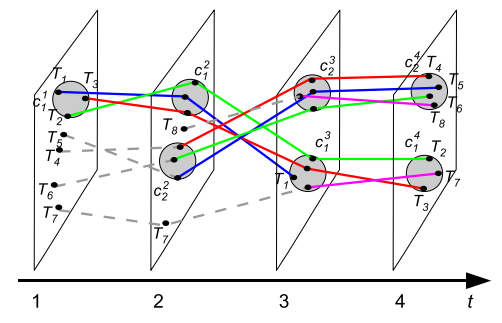
\includegraphics[scale=0.8]{flp}  
	\caption{Ilustrasi \textit{flock pattern} menurut \cite{flock_pattern_1:16}} 
	\label{fig:flp} 
\end{figure}

\section{Basic Flock Evaluation Algorithm}
\label{sec:bfe}

\par Misalkan trajektori $T_{id}$ merepresentasikan pergerakan sebuah objek dengan $id$ tertentu ($O_{id}$) yang bergerak pada suatu bidang. Trajektori $T_{id}$ terdiri dari $n$ buah titik $p(t_i)$.
\begin{equation}\label{definisi_trajektori}
	T_{id}=\{p(t_{1}),p(t_{2}),\cdots ,p(t_{n})\}
\end{equation}
Titik $p(t_i)$ adalah lokasi objek $O_{id}$ pada ruang dua dimensi $\mathbb{R}^2$ pada waktu $t_i$. Titik-titik tersebut terurut berdasarkan \textit{timestamp} $t_i (t_i\in N, t_{i-1} < t_i, 0 < i \leq n)$. Sedangkan $L_p$ menyatakan jarak di antara dua titik $p_a^{t_i}$ dan $p_b^{t_i}$ pada waktu $t_i$ yang dihitung oleh fungsi $d(p_a^{t_i},p_b^{t_i})$ menggunakan metrik tertentu.

\par Salah satu masalah utama pada algoritma \textit{basic flock evaluation} adalah titik pusat sebuah \textit{flock} pada \textit{flock pattern} tidak selalu terletak pada trajektori. Karena jumlah titik lokasi trajektori ($p_{id}$) terlalu banyak maka tidak mungkin untuk memeriksa seluruh titik tersebut secara satu per satu. Maka sebuah teorema digunakan untuk membatasi ukuran ruang pencarian. 

\par \textbf{Teorema 1}: Jika untuk setiap waktu $t_i$ terdapat sebuah titik $c_k^{t_i}$ pada ruang sedemikian rupa sehingga $\forall T_{j}\in f,d(p_j^{t_i},c_k^{t_i})\leq\epsilon/2 $, maka terdapat titik lain ($c`_k^{t_i}$) yang memenuhi $\forall T_{j}\in f,d(p_j^{t_i},c`_k^{t_i})\leq\epsilon/2 $ dan terdapat trajektori $T_{a}\in f$ dan $T_{b}\in f$ sehingga $\forall T_j\in\{T_a,T_b\},d(p_j^{t_i},c`_k^{t_i})=\epsilon/2 $.

\par Teorema tersebut menjelaskan jika terdapat sebuah cakram $c_k^{t_i}$ dengan diameter $\epsilon$ yang mencakup seluruh trajektori pada \textit{flock} $f$ pada waktu $t_i$, maka terdapat cakram lain dengan diameter yang sama namun memiliki titik pusat yang berbeda yaitu $c`_k^{t_i}$ yang juga mencakup seluruh trajektori pada cakram pertama (gambar \ref{fig:proof}). Pada garis keliling (\textit{circumference}) kedua cakram tersebut terdapat minimal dua titik lokasi trajektori.

\begin{figure}[H]
	\centering  
	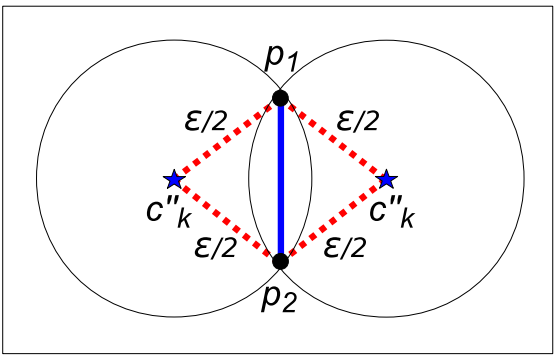
\includegraphics[scale=0.4]{fig5}  
	\caption{Cakram yang menyinggung titik $p_1$ dan $p_2$ pada garis kelilingnya dengan $d(p_1,p_2)\leq\epsilon$} 
	\label{fig:theorem1} 
\end{figure}

\par Misalkan terdapat sebuah cakram (atau lingkaran) dengan diameter $\epsilon$ dan berpusat di $c_k$ yang mencakup seluruh trajektori pada flock pada waktu $t_i$ (gambar \ref{fig:proof}(a)). Asumsikan tidak ada trajektori yang terletak pada garis batas cakram sehingga $\forall T_j \in f, d(T_j ,c_k) < \epsilon/2$. Dari cakram ini dapat ditemukan cakram lain yang memeiliki sifat yang sama namun memiliki titik pusat yang berbeda. Cakram tersebut dibentuk dengan melakukan translasi dan rotasi pada cakram yang berpusat di $c_k$. 

\begin{figure}[H]
	\centering  
	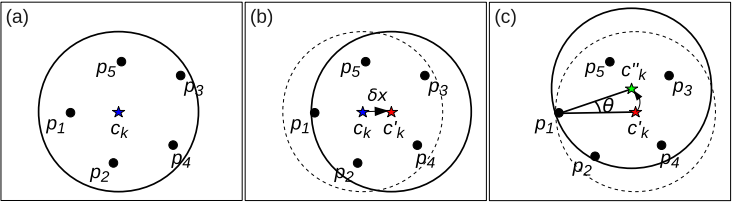
\includegraphics[scale=0.6]{fig4}  
	\caption{Pembuktian teorema 1} 
	\label{fig:proof} 
\end{figure}

\par Langkah pertama adalah titik $c_k$ digeser searah sumbu x hingga trajektori yang terletak di paling kiri \textit{flock} berada di garis keliling lingkaran (gambar \ref{fig:proof}(b)). Pada gambar \ref{fig:proof}(b), titik (lokasi tertentu pada trajektori) pertama yang bersinggungan dengan garis keliling cakram setelah titik pusat cakram digeser adalah $p_1$. Titik pusat cakram kini berpindah ke $c`_k$ dan seluruh titik pada \textit{flock} berada dalam radius cakram baru yang berpusat di $c`_k$.

\par Langkah kedua adalah cakram yang baru dibentuk diputar dengan menggunakan titik $p_1$ sebagai titik pusat putaran. Cakram tersebut diputar hingga titik lain ($p_2$) bersinggungan dengan garis kelilingnya (gambar \ref{fig:proof}(c)). Sehingga terbentuk cakram baru yang mencakup seluruh titik pada \textit{flock} yang berpusat di $c^{``}_k$ dengan diameter $\epsilon$. Cakram yang baru terbentuk memiliki minimal dua titik pada garis kelilingnya.

\par Teorema ini membatasi ukuran ruang pencarian lokasi \textit{flock} pada domain spasial. Pada himpunan yang berisi $|T|$ buah trajektori terdapat $|T|^2$ kemungkinan pasangan kombinasi titik pada waktu tertentu. Setiap pasangan titik memiliki tepat dua cakram dengan radius $\epsilon/2$ dan kedua titik tersebut terletak pada garis keliling kedua cakram (gambar \ref{fig:theorem1}). Setiap cakram minimal memiliki $\mu$ buah trajektori. Untuk setiap \textit{time instance} pada interval waktu $\delta$ terdapat $2|T|^2$ \textit{flock pattern} yang mungkin. Banyaknya flock pattern yang mungkin adalah $2|T|^{2\delta}$. Sehingga \textit{flock pattern problem} pada \textit{fixed time duration} memiliki kompleksitas waktu polinomial yaitu $O(|T|^{|\delta|})$ \cite{flock_pattern_discovery_2:09}.

\subsection{\textit{Reporting Flock Pattern}}
\par Untuk menghitung flock disks secara efisien, digunakanlah struktur berbasis grid(\textit{grid-based structure}). Struktur berbasis grid yang digunakan terdiri dari kumpulan \textit{grid cell} dengan panjang sisi $\epsilon$. Setiap titik lokasi pada trajektori $T_{id}$ pada waktu $t_i$, yaitu ($p_{id}^{t_i}$) terletak pada \textit{grid cell} tertentu. Pilihan \textit{grid cell} yang digunakan ditentukan oleh \textit{latitude} dan \textit{longitude} $p_{id}^{t_i}$. Setiap titik lokasi hanya dimasukkan ke satu \textit{grid cell}. Jumlah total \textit{grid cell} pada \textit{grid index} dipengaruhi oleh distribusi trajektori pada waktu tertentu ($t_{i}$) dan nilai $\epsilon$. Semakin kecil nilai $\epsilon$, semakin besar jumlah \textit{grid cell} yang dibutuhkan. 

\par Menurut implementasi yang diusulkan oleh Vieira .et al \cite{flock_pattern_discovery_2:09}, \textit{grid cell} yang kosong tidak digunakan. Sebuah struktur data digunakan untuk menyimpan trajektori pada \textit{grid cell}. Jika nilai $\epsilon$ tidak terlalu besar, maka jumlah titik pada setiap \textit{grid cell} relatif sedikit sehingga struktur data sederhana seperti \textit{list} dapat digunakan. Ilustrasi \textit{grid-based index} ditunjukkan oleh gambar \ref{fig:gidx}.

\begin{figure}[H]
	\centering  
	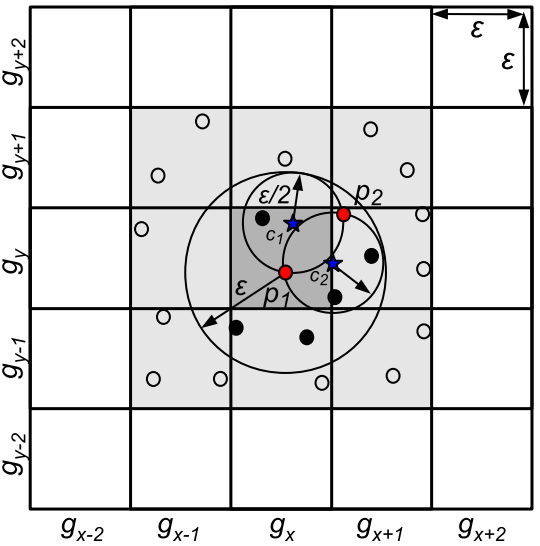
\includegraphics[scale=0.5]{fig6}  
	\caption{Ilustrasi \textit{grid-based index}. Setiap \textit{grid cell} pada indeks memiliki sisi sepanjang $\epsilon$ dan berisi kumpulan titik lokasi ($p_{id}^{t_i}$). \textit{grid cell} yang diarsir abu gelap adalah \textit{grid cell} yang sedang diproses ($g_{x,y}$). Sedangkan \textit{grid cell} yang diarsir abu terang adalah \textit{grid cell} yang bertetangga dengan $g_{x,y}$. Titik-titik berwarna hitam adalah titik-titik yang terletak pada radius $\epsilon$ dari titik $p_1$ (baris 8 algoritma 1). Titik $p_1$ adalah titik pada $g_{x,y}$ yang saat ini sedang diproses (baris 7 algoritma 1). Titik-titik yang berwarna merah adalah pasangan titik yang jaraknya $\leq\epsilon$ (baris 11 algoritma 1). Bintang berwarna biru menyatakan titik pusat dua lingkaran yang dihasilkan dari pasangan titik $p_1$ dan $p_2$. Lingkaran $c_1$ dan $c_2$ adalah kandidat \textit{disk} pada \textit{flock} untuk waktu $t_i$} 
	\label{fig:gidx} 
\end{figure}

\par Setelah struktur \textit{grid index} untuk waktu $t_i$ selesai dihitung, Algoritma 1 dapat digunakan untuk memproses cakram-cakram yang dihasilkan. Untuk setiap \textit{grid cell} $g_{x,y}$, hanya sembilan $grid cell$ yang bertetangga dengan $g_{x,y}$ dan $g_{x,y}$ itu sendiri yang harus diproses. Algoritma 1 memproses setiap titik lokasi pada \textit{grid cell} $g_{x,y}$ maupun titik lokasi pada \textit{grid cell} pada rentang $[g_{x-1,y-1}\cdots g_{x+1,y+1}]$ untuk menemukan pasangan titik $p_r$ dan $p_s$ dengan jarak diantara kedua titik tersebut tidak lebih dari $\epsilon$ ($d(p_r,p_s)\leq\epsilon$). Karena seluruh grid cell pada indeks memiliki ukuran $\epsilon$, grid cell yang terletak di luar rentang $[g_{x-1,y-1}\cdots g_{x+1,y+1}]$ tidak perlu diperiksa. Pasangan titik yang belum diproses saat ini dan memiliki jarak tidak lebih dari $\epsilon$ satu sama lain akan digunakan untuk menghitung dua cakram $c_1$ dan $c_2$. Jika jarak antara pasangan titik $p_r$ dan $p_s$  tepat sama dengan $\epsilon$, maka cakram $c_1$ dan $c_2$ memiliki pusat yang sama sehingga hanya salah satu cakram yang perlu diproses.

\begin{algorithm}
\caption{ Menghitung \textit{disk} pada \textit{grid-based index}}
\begin{algorithmic}[1]
\State $\mathcal{C}\gets\emptyset$
\State $Index.Build(\mathcal{T}[t_i],\epsilon)$
\For{setiap \textit{grid cell} yang tidak kosong $g_{x,y}\in Index$}
	\State $P_r\gets g_{x,y}$
	\State $P_s\gets [g_{x-1,y-1}\cdots g_{x+1,y+1}]$
	\If{$|P_s|\geq\mu$}
		\For{each $p_r\in P_r$}
		\State $\mathcal{H}\gets Range(p_r,\epsilon)$
			\For{each $p_j\in\mathcal{H}$}
				\If{not computed$\{p_r,p_j\}$ yet}
					\State compute disks $\{c_1,c_2\}$ defined by $\{p_r,p_j\}$ and diameter $\epsilon$
					\For{each disk $c_k\in\{c_1,c_2\}$}
					\State $c\gets c_k\cap\mathcal{H}$
					\If{$|c|\geq\mu$}
						\State $\mathcal{C}.Add(c)$
					\EndIf
					\EndFor
				\EndIf
			\EndFor
		\EndFor
	\EndIf
\EndFor\\
\Return $\mathcal{C}$
\end{algorithmic}
\end{algorithm}

\par Tidak semua titik pada rentang $[g_{x-1,y-1}\cdots g_{x+1,y+1}]$ dapat dipasangkan dengan titik-titik pada $g_{x,y}$. Hanya pasangan titik yang memiliki jarak $d(p_r,p_s)\leq\epsilon$. Langkah berikutnya adalah memeriksa posisi titik-titik hasil \textit{range query} jikalau titik-titik tersebut berada di dalam cakram yang dihitung pada tahap sebelumnya. Untuk setiap titik $p_r$ pada \textit{grid cell} $g_{x,y}$, sebuah \textit{range query} dengan radius $\epsilon$ dilakukan pada seluruh \textit{grid} $[g_{x-1,y-1}\cdots g_{x+1,y+1}]$ untuk menemukan titik-titik yang bisa dipasangkan dengan titik $p_r$ sehingga $d(p_r,p_s)\leq \epsilon$ terpenuhi (gambar \ref{fig:fig7}(a)). Hasil dari \textit{range query} disimpan pada \textit{list} $\mathcal{H}$ yang digunakan untuk memeriksa cakram yang dihitung. Untuk setiap pasangan titik yang valid, terdapat dua cakram yang dihasilkan. Untuk setiap cakram yang dihasilkan, titik-titik pada list $\mathcal{H}$ diperiksa jikalau mereka terletak di dalam cakram (gambar \ref{fig:fig7}(b)). Cakram yang jumlah titiknya kurang dari $\mu$ dibuang. Sedangkan cakram yang jumlah titiknya $\geq\mu$ disimpan. Pada gambar \ref{fig:fig7}(c), cakram $c_1$ dibuang dan cakram $c_2$ dianggap valid.

\begin{figure}[H]
	\centering  
	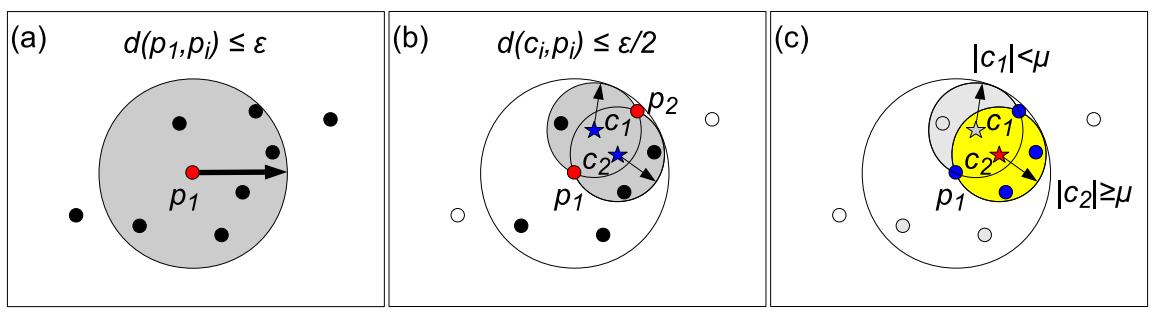
\includegraphics[scale=0.5]{fig7}  
	\caption{Proses menemukan \textit{flock} pada waktu $t$.} 
	\label{fig:fig7} 
\end{figure}

\par Jika terdapat dua cakram valid dengan elemen yang hampir sama, maka cakram dengan jumlah titik terbanyak yang akan dipilih. Algoritma 1 menerapkan hal ini dengan cara membandingkan titik pusat cakram dan jumlah total elemen yang sama pada setiap cakram. Sebuah cakram $c_1$ diperiksa dengan cakram lain $c_2$ jika jarak keduanya tidak lebih dari $\epsilon$ ($d(c_1,c_2)\leq\epsilon$). Jika sebaliknya, maka dua cakram tidak memiliki elemen yang sama. Agar operasi tersebut berjalan dengan seefisien mungkin, titik tengah dan jari-jari $\epsilon/2$ seriap cakram disimpan pada struktur data \textit{k-d-tree}. Untuk setiap cakram $c_1$ algoritma akan membandingkannya dengan elemen-elemen pada \textit{k-d-tree} untuk mencari cakram yang bersinggungan dengan $c_1$. Karena titik-titik milik sebuah cakram disimpan dalam \textit{binary tree}, operasi mencari \textit{subset} atau \textit{superset} dapat dilakukan dengan efisien. Karena itu, elemen yang sama pada dua cakram dapat dicari dengan memeriksa (\textit{scan}) setiap elemen pada kedua cakram tepat satu kali. Jika kardinalitas dari elemen yang sama pada cakram $c_1$ dan $c_2$ sama dengan kardinalitas elemen $c_1$ ($|c_1\cap c_2|=c_1$), maka $c_1\subset c_2$ sehingga cakram $c_1$ dapat dibuang. Jika $|c_1\cap c_2|=|c_2|$, maka cakram $c_2$ dapat dibuang. Jika $|c_1\cap c_2|\neq|c_2|$ dan $|c_1\cap c_2|\neq|c_1|$, maka cakram $c_1$ dan $c_2$ disimpan ke dalam $\mathcal{C}$. 

\par Pada algoritma \textit{basic flock pattern evaluation}(BFE), sebuah kandidat \textit{disk} dihitung untuk setiap \textit{time instance} $t_i$, dimulai dari \textit{time instance} pertama ($t_1$) dan terus berlanjut sampai \textit{time instance} terakhir. Setiap kandidat \textit{disk} yang dihasilkan untuk setiap \textit{time instance} $t_i$ dianalisa dan digabungkan(\textit{join}) dengan kandidat \textit{flock} yang dihasilkan pada waktu sebelumnya ($t_{i-1}$). Hanya \textit{flock} yang sukses digabungkan dengan \textit{disk} saat ini yang dipertahankan. Algoritma BFE mengembalikan sebuah \textit{flock pattern} yang memenuhi syarat temporal $\delta$, yaitu setiap \textit{flock} memiliki $\delta$ buah \textit{disk}.

\par \textit{disk} yang dihasilkan untuk \textit{time instance} pertama oleh \textit{grid index} dianggap sebagai \textit{flock} parsial yang disimpan pada \textit{list}. \textit{list} tersebut berisi kandidat \textit{flock} pada waktu saat ini ($\mathcal{F}^{t_i}$). Pada \textit{time instance} selanjutnya, \textit{disk}-\textit{disk} yang dihasilkan oleh \textit{grid-based index} disimpan dalam \textit{list} kandidat \textit{flock} $\mathcal{F}^{t_i}$ dan digabungkan dengan kandidat \textit{flock} pada waktu sebelumnya ($\mathcal{F}^{t_{i-1}};\mathcal{F}^{t_i}=\mathcal{F}^{t_i}\cap\mathcal{F}^{t_{i-1}}$). $\mathcal{F}^{t_i}$ dapat digabungkan dengan $\mathcal{F}^{t_{i-1}}$ jika jumlah total elemen yang sama di antara kandidat \textit{flock} dan \textit{disk} tidak kurang dari $\mu$ ($|c\cap f|\geq\mu$).

\par Jika kondisi tersebut terpenuhi, maka hasil penggabungan ditambahkan ke dalam \textit{list} kandidat \textit{flock} untuk waktu $t_i$. Sebuah kandidat \textit{flock} dianggap valid jika terdapat minimal $\delta$ buah operasi penggabungan(\textit{join}). $\mathcal{F}^{t_i}$ hanya menyimpan \textit{flock} yang dimulai pada waktu sebelumnya ($t_{start}>t_i-\delta$) dan berakhir pada waktu saat ini ($t_{end}=t_i$). \textit{disk-disk} yang tidak dapat digabungkan dibuang.

\par Keunggulan algoritma BFE adalah untuk setiap \textit{time instance} yang sedang diproses, $\mathcal{F}^{t_i}$ hanya menyimpan id trajektori. Selain itu, lokasi trajektori untuk setiap \textit{time instance} hanya diproses sekali sehingga data trajektori pada \textit{time window} yang panjangnya $\delta$ tidak perlu di-\textit{buffer} \cite{flock_pattern_discovery_2:09}.

\begin{algorithm}
\caption{\textit{Basic Flock Evaluation}}
\begin{algorithmic}[1]
\State $\mathcal{F}^{t_0}\gets\emptyset$ \Comment{Inisialisasikan \textit{flock} parsial}
\For{each \textit{time instance} $t_i$}
	\State $\mathcal{L}\gets\mathcal{T}[t_i]$ \Comment{lokasi-lokasi yang terletak pada trajektori pada waktu $t_is$}
	\State $\mathcal{C}\gets Index.Disks()$ \Comment{Hitung kandidat \textit{disk} untuk waktu $t_i$ dengan menggunakan algoritma 1}
	\State $\mathcal{F}^{t_i}\gets\emptyset$ \Comment{Untuk menyimpan kandidat \textit{flock} yang potensial}
	\For{each $c\in\mathcal{C}$}
		\For{each $f\in\mathcal{F}^{t_{i-1}}$} \Comment{\textit{flock} sebelumnya yang berpotensi}
			\If{$|c\cap f|\geq\mu$}
				\State $u\gets c\cap f$
					\State $u.t_{start}\gets f.t_{start}$ \Comment{tetapkan waktu mulai}
					\State $u.t_{end}\gets t$ \Comment{tetapkan waktu akhir}
					\If{$u.t_{end}-u.t_{start}=\delta$} \Comment{jika \textit{flock} ditemukan}
						\State report \textit{flock pattern} $u$ from $u.t_{start}$ to $u.t_{end}$
						\State update $u.t_{start}$
						\State $\mathcal{F}^{t_i}\gets\mathcal{F}^{t_i}\cup u$ \Comment{tambahkan \textit{flock} $u$}
					\EndIf
			\EndIf
			\State $\mathcal{F}^{t_i}\gets\mathcal{F}^{t_i}\cup c$ \Comment{tambahkan \textit{disk} $c$ kedalam $\mathcal{F}^{t_i}$}
		\EndFor
	\EndFor
\EndFor
\end{algorithmic}
\end{algorithm}

\subsection{Filter flock disks}
\par Jumlah kandidat \textit{disk} untuk \textit{time instance} tertentu bisa saja terlalu banyak sehingga \textit{cost} untuk melakukan \textit{join} kandidat \textit{disk} ke \textit{flock pattern} terlalu tinggi. Terdapat empat heuristik untuk mengatasi masalah ini yaitu:

\begin{enumerate}
\item \textit{Top Down Evaluation} (TDE)\\
Berbeda dengan algoritma BFE yang menyusun \textit{flock} secara \textit{bottom-up} yaitu menyusun \textit{flock} secara satu per satu mulai dari \textit{time instance} pertama, TDE menyusun \textit{flock} secara \textit{top-down}. Metode \textit{top-down} membandingkan kandidat \textit{disk} pada dua \textit{time instance} yang berjarak $\delta$ \textit{time instance} satu sama lain. Metode ini didasarkan pada asumsi bahwa dua kandidat \textit{disk} pada dua \textit{time instance} yang berurutan 
 memiliki perbedaan yang sedikit sedangkan dua kandidat \textit{disk} yang berjarak $\delta$ \textit{time instance} memiliki perbedaan yang signifikan. Perbedaan antara dua kandidat \textit{disk} pada dua \textit{time instance} yang berurutan menghasilkan \textit{flock} pendek dalam jumlah besar sedangkan perbedaan antara dua kandidat \textit{disk} yang berjarak $\delta$ \textit{time instance} menghasilkan kandidat \textit{flock} dalam jumlah kecil.
 
 \par Heuristik ini mem-\textit{buffer} lokasi trajektori untuk \textit{time window} $w$ yang memiliki panjang $\delta$ \textit{time instance}. Untuk menggabungkan \textit{disk} dengan kandidat \textit{flock}, pertama-tama kandidat \textit{disk} $\mathcal{C}^1$ untuk \textit{time instance} pertama $t_{i-\delta+1}$ pada \textit{window} $w$ dihitung. Lalu, \textit{disk} untuk \textit{time instance} terakhir $t_i$ pada $w$ dihitung dan digabungkan dengan \textit{disk} pada $\mathcal{C}^1$. Kandidat \textit{flock} untuk \textit{time window} $w$ yang dihasilkan kemudian diverifikasi dengan menggunakan algoritma BFE.

\item \textit{Pipe Filter Evaluation} (PFE)\\
Heuristik kedua menggunakan paradigma \textit{filter and refine}. Heuristik akan memilih trajektori-trajektori yang memiliki minimal $\mu$ buah entitas yang berada dalam radius $\epsilon$ selama minimal $\delta$ satuan waktu. Lalu \textit{flock pattern} dicari menggunakan algoritma BFE. Pada heuristik PFE, sebuah \textit{grid-based index} untuk \textit{time instance} $t_{i-\delta}$ pada \textit{time window} $w$ dihitung. Lalu, operasi \textit{range search} dilakukan pada setiap trajektori $T_j$ pada waktu $t_{i-\delta}$. Tujuan kueri tersebut adalah memeriksa jumlah lokasi objek lain yang berada pada radius $\epsilon$ dari trajektori yang sedang diproses. 

\par Jika kardinalitas dari hasil operasi \textit{range search} lebih besar atau sama dengan $\mu$, maka operasi serupa dilakukan pada \textit{time instance} $t_{i-\delta}$ hingga $t_i$. Jika total jumlah trajektori di dalam "pipa" yang terbentuk untuk setiap trajektori $T_j$ adalah $|\mathcal{U}|\geq\mu$, maka trajektori tersebut ditambahkan kedalam \textit{list} kandidat $\mathcal{M}$ untuk diproses lebih lanjut pada tahap \textit{refinement}.

\par Tahap \textit{refinement} menggunakan algoritma BFE dan hanya memproses trajektori hasil tahap \textit{filter} ($\mathcal{M}$). Berbeda dengan algoritma BFE yang memproses seluruh trajektori yang tersimpan. Metode ini digunakan jika \textit{cost} untuk menghitung kandidat \textit{disk} adalah \textit{computationally expensive} dan konstruksi \textit{flock} dilakukan pada \textit{subset} trajektori. Gambar \ref{fig:fig8} mengilustrasikan \textit{pipe} yang terbentuk  untuk trajektori $T_2$ pada waktu $\delta$ dalam radius $\epsilon$.
\begin{figure}[H]
	\centering  
	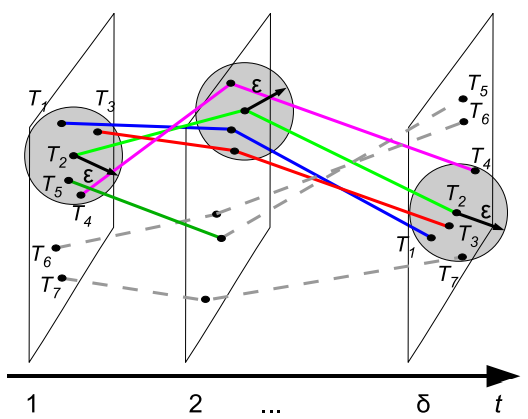
\includegraphics[scale=0.5]{fig8}  
	\caption{\textit{pipe filtering} untuk trajektori $T_2$ pada waktu $\delta$ dalam radius $\epsilon$} 
	\label{fig:fig8} 
\end{figure} 

\item \textit{Continuous Refinement Evaluation} (CRE)\\
Heuristik ini terus-menerus memurnikan kumpulan trajektori yang dapat menjadi bagian sebuah \textit{flock pattern} (\textit{continuous refinement}). Metode ini menggunakan tahap \textit{disk generation} untuk \textit{time instance} $t_i$ sebagai tahap \textit{filtering} untuk \textit{time instance} $t_{i+1}$. Hanya trajektori yang berada dalam kandidat \textit{disk} pada waktu $t_i$ yang akan dianalisis pada waktu $t_{i+1}$. Metode ini digunakan pada situasi dengan selektivitas kandidat \textit{disk} tinggi. Contohnya pada kandidat \textit{disk} dalam jumlah kecil dan jumlah trajektori pada kandidat \textit{disk} juga tidak banyak.

\par Tahap pertama pada \textit{continuous refinement} adalah mencari semua \textit{disk} $\mathcal{C}^1$ menggunakan lokasi-lokasi $\mathcal{L}[1]$ untuk \textit{time instance} $t_{i-\delta}$. Lalu, untuk setiap cakram $c^1,c^1\in \mathcal{C}^1$, trajektori yang berada di dalamnya diproses lebih lanjut dari waktu $t_{i-\delta+1}$ hingga $t_i$.

\par Pada \textit{time instance} pertama, \textit{disk} $\mathcal{C}^1$ untuk \textit{time instance} $t_{i-\delta}$ disimpan dalam $\mathcal{F}^1$. Lalu, setiap objek $c_1$ diproses lebih lanjut untuk menghitung \textit{disk} lalu di-\textit{merge-join} dengan \textit{disk} milik \textit{time instance}sebelumnya yang disimpan di $\mathcal{F}^t$. Jika $\mathcal{F}^t$ tidak memiliki kandidat \textit{flock} yang potensial	pada waktu $t$, maka pemrosesan $c^1$ dapat dihentikan. Setelah langkah ini, \textit{flock pattern} untuk waktu $t_{i-\delta}$ hingga $t_i$ selesai dihitung. 


\item \textit{Cluster Filtering Evaluation} (CFE)\\
Terdiri dari dua tahap utama. Pertama-tama algoritma \textit{DBSCAN Clustering} dengan parameter $eps=\epsilon$ dan $minPts=\mu$ untuk setiap \textit{time instance} $t_i$. \textit{Cluster} yang ditemukan untuk setiap \textit{time instance} lalu digabungkan dengan \textit{cluster} yang ditemukan pada $t_{i-1}$. Dua \textit{cluster} dapat digabungkan jika memiliki minimal $\mu$ buah trajektori yang sama. Jika \textit{cluster} $u$ dapat disusun dengan cara yang disebutkan untuk $\delta$ buah \textit{time instance} yang berturut-turut, maka $u$ dianggap sebagai kandidat \textit{disk} yang valid. Kemudian kandidat \textit{disk} tersebut diproses menggunakan algoritma BFE.

\par Gambar \ref{fig:fig9} mengilustrasikan langkah-langkah pada algoritma CFE. Pada gambar \ref{fig:fig9}(a) operasi DBSCAN dilakukan pada objek lokasi (titik) tertentu ($p_1$) dengan parameter $eps=\epsilon$ dan $minPts=\mu$. Lalu, pada gambar \ref{fig:fig9}(b), operasi DBSCAN dilakukan pada titik-titik yang bertetangga dengan $p_1$. Titik yang tidak berada dalam \textit{cluster}. \textit{Cluster} yang terbentuk oleh operasi DBSCAN (gambar \ref{fig:fig9}(c)) diproses lebih lanjut pada tahap \textit{refinement}.

\begin{figure}[H]
	\centering  
	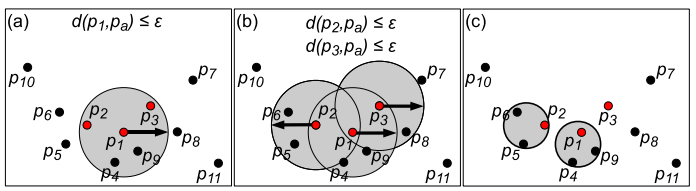
\includegraphics[scale=0.5]{fig9}  
	\caption{Ilustrasi proses pembentukan \textit{cluster} pada algoritma CFE} 
	\label{fig:fig9} 
\end{figure} 

\end{enumerate}

\par Kesimpulannya, algoritma BFE memiliki tiga tahapan utama yaitu mencari kandidat-kandidat \textit{disk} dengan bantuan \textit{grid-based index}, memilih kandidat \textit{disk} dengan jumlah trajektori yang maksimal, dan menggabungkan \textit{flock} pada waktu saat ini dengan \textit{flock} pada waktu sebelumnya \cite{flock_pattern_1:16}.
 
\section{Spatial Data Types}
Secara umum, terdapat tiga jenis data spasial yang digunakan untuk merepresentasikan suatu objek geografi yaitu \textit{point} (titik), \textit{line}, dan \textit{region}. Setiap jenis data tersebut dibagi lagi ke dalam dua kelas yaitu \textit{simple} dan \textit{complex} \cite{advdb:15}. Ilustrasi \textit{simple point, line}, dan \textit{region} ditunjukkan oleh gambar \ref{fig:simple}. Ilustrasi \textit{complex point, line}, dan \textit{region} ditunjukkan oleh gambar \ref{fig:complex}.
\begin{enumerate}
\item \textit{simple point}\\
adalah sebuah titik yang terletak pada ruang dua dimensi.

\item \textit{simple line}\\
adalah sebuah objek satu dimensi pada ruang dua dimensi yang memiliki dua ujung.

\item \textit{simple region}\\
adalah kurva tertutup sederhana yang memisahkan sebuah bidang menjadi dua bagian yaitu bagian dalam dan bagian luar.

\item \textit{complex point}\\
kumpulan simple point yang tidak saling tumpang tindih.

\item \textit{complex line}\\
adalah kumpulan garis sederhana yang saling lepas.

\item \textit{complex region}\\
Adalah kumpulan \textit{face} dan  \textit{hole}. \textit{Face} adalah region sederhana yang memiliki beberapa \textit{hole}. \textit{Hole} memenuhi kriteria \textit{simple region} tetapi bagian dalam sebuah \textit{complex region} berada di bagian luar \textit{hole} dan bagian luarnya berada di bagian dalam \textit{hole}. Batas–batas \textit{face} dan \textit{hole} bisa saling bersentuhan pada titik-titik diskrit yang terbatas.

\end{enumerate}

\begin{figure}[H]
\centering  
	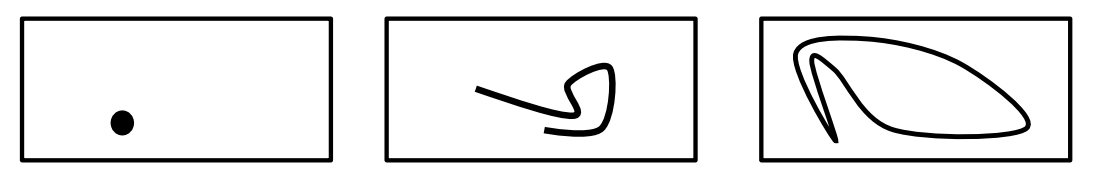
\includegraphics[scale=0.5]{simple}  
	\caption{Ilustrasi \textit{simple point} (kiri), \textit{simple line} (tengah), dan \textit{simple region} (kanan)} 
	\label{fig:simple} 
\end{figure}

\begin{figure}[H]
\centering  
	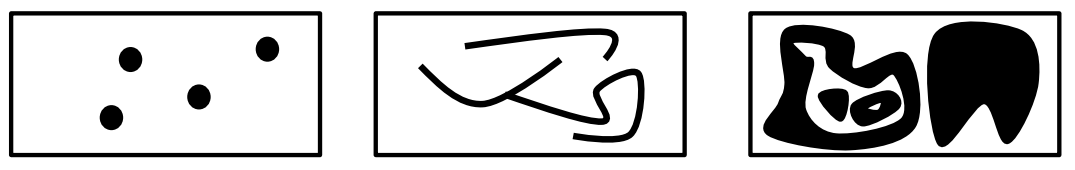
\includegraphics[scale=0.5]{complex}  
	\caption{Ilustrasi \textit{complex point} (kiri), \textit{complex line} (tengah), dan \textit{complex region} (kanan)} 
	\label{fig:complex} 
\end{figure}